
%%%%%%%%%%%%%%%%%%%%%%%%%%%%%%%%%%%%%%%%%%%%%%%%%%%%%%%%%%%%%%%%%%%%%%%%%%%%%%%%%%%%%%%
%%%%%%%%%%%%%%%%%%%%%%%%%%%%%%%%%%%%%%%%%%%%%%%%%%%%%%%%%%%%%%%%%%%%%%%%%%%%%%%%%%%%%%%
% 
% This top part of the document is called the 'preamble'.  Modify it with caution!
%
% The real document starts below where it says 'The main document starts here'.

\documentclass[12pt]{article}

\usepackage{amssymb,amsmath,amsthm}
\usepackage[top=1in, bottom=1in, left=1.25in, right=1.25in]{geometry}
\usepackage{fancyhdr}
\usepackage{enumerate}
\usepackage{listings}
\usepackage{graphicx}
\usepackage{float}
\usepackage{multirow}

\usepackage{mwe}
\usepackage{caption}
\usepackage{subcaption}
% Comment the following line to use TeX's default font of Computer Modern.
\usepackage{times,txfonts}



\makeatletter
\renewcommand*\env@matrix[1][*\c@MaxMatrixCols c]{%
  \hskip -\arraycolsep
  \let\@ifnextchar\new@ifnextchar
  \array{#1}}
\makeatother

\newtheoremstyle{homework}% name of the style to be used
  {18pt}% measure of space to leave above the theorem. E.g.: 3pt
  {12pt}% measure of space to leave below the theorem. E.g.: 3pt
  {}% name of font to use in the body of the theorem
  {}% measure of space to indent
  {\bfseries}% name of head font
  {:}% punctuation between head and body
  {2ex}% space after theorem head; " " = normal interword space
  {}% Manually specify head
\theoremstyle{homework} 

% Set up an Exercise environment and a Solution label.
\newtheorem*{exercisecore}{Exercise \@currentlabel}
\newenvironment{exercise}[1]
{\def\@currentlabel{#1}\exercisecore}
{\endexercisecore}

\newcommand{\localhead}[1]{\par\smallskip\noindent\textbf{#1}\nobreak\\}%
\newcommand\solution{\localhead{Solution:}}

%%%%%%%%%%%%%%%%%%%%%%%%%%%%%%%%%%%%%%%%%%%%%%%%%%%%%%%%%%%%%%%%%%%%%%%%
%
% Stuff for getting the name/document date/title across the header
\makeatletter
\RequirePackage{fancyhdr}
\pagestyle{fancy}
\fancyfoot[C]{\ifnum \value{page} > 1\relax\thepage\fi}
\fancyhead[L]{\ifx\@doclabel\@empty\else\@doclabel\fi}
\fancyhead[C]{\ifx\@docdate\@empty\else\@docdate\fi}
\fancyhead[R]{\ifx\@docauthor\@empty\else\@docauthor\fi}
\headheight 15pt

\def\doclabel#1{\gdef\@doclabel{#1}}
\doclabel{Use {\tt\textbackslash doclabel\{MY LABEL\}}.}
\def\docdate#1{\gdef\@docdate{#1}}
\docdate{Use {\tt\textbackslash docdate\{MY DATE\}}.}
\def\docauthor#1{\gdef\@docauthor{#1}}
\docauthor{Use {\tt\textbackslash docauthor\{MY NAME\}}.}
\makeatother

% Shortcuts for blackboard bold number sets (reals, integers, etc.)
\newcommand{\Reals}{\ensuremath{\mathbb R}}
\newcommand{\Nats}{\ensuremath{\mathbb N}}
\newcommand{\Ints}{\ensuremath{\mathbb Z}}
\newcommand{\Rats}{\ensuremath{\mathbb Q}}
\newcommand{\Cplx}{\ensuremath{\mathbb C}}
%% Some equivalents that some people may prefer.
\let\RR\Reals
\let\NN\Nats
\let\II\Ints
\let\CC\Cplx
%%%%%%%%%%%%%%%%%%%%%%%%%%%%%%%%%%%%%%%%%%%%%%%%%%%%%%%%%%%%%%%%%%%%%%%%%%%%%%%%%%%%%%%
%%%%%%%%%%%%%%%%%%%%%%%%%%%%%%%%%%%%%%%%%%%%%%%%%%%%%%%%%%%%%%%%%%%%%%%%%%%%%%%%%%%%%%%
% 
% The main document start here.

% The following commands set up the material that appears in the header.
\doclabel{Stat 605: Homework 3}
\docauthor{Stefano Fochesatto}
\docdate{\today}

\begin{document}

\begin{exercise}{1} Use the following r code to simulate and plot a data set 
  consisting of $n = 60$ values from the model $Y = \beta_0 + \beta_1 X_1 + 
  \beta_2 X_2 + \epsilon$, where the $\epsilon$'s  are independent $N(0,\sigma ^2)$
  random variables.\\
  \textbf{Code:}
        \begin{center}
        \lstinputlisting[basicstyle = \footnotesize]{r1.r}
        \end{center}
\begin{enumerate}
  \item[a.] Include the resulting plot in your write-up.\\
  \solution Running the given R code produces the following plot,
  \begin{figure}[H]
    \begin{center}
    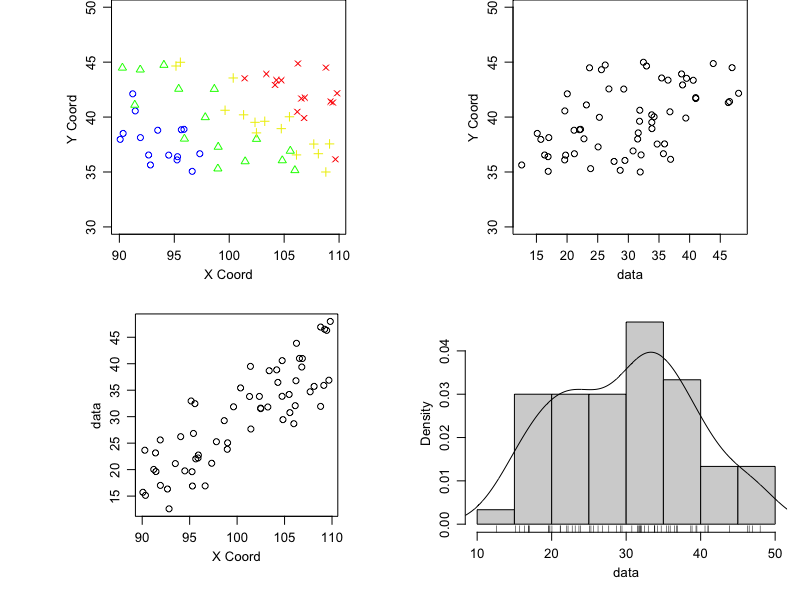
\includegraphics[width = \textwidth]{Rplot.png}
    \end{center}
  \end{figure}
  \vspace{.15in} 




  \item[b.] What are the values of $\beta_0$, $\beta_1$, $\beta_2$, and $\sigma^2$ 
  that are being used to simulate these data?\\
  \solution The given R code defines the following function for $Y$ (assuming $lons = X_1$ and $lat = X_2$),
  \begin{align*}
    Y &= 30 + 1.3(X_1 - 100) + 1.5(X_2 - 40) + \epsilon,\\
      &= 30 + 1.3X_1 - 130 + 1.5X_2 - 60 + \epsilon,\\
      &= -160 + 1.3X_1 + 1.5X_2 + \epsilon.
  \end{align*}
  Simplifying the function we get that $\beta_0 = -160$, $\beta_1 = 1.3$, $\beta_2 = 1.5$. The distribution of $\epsilon$ is 
  described by the rnorm() function which gives $\sigma^2 = 1.6^2 = 2.56$.
  \vspace{.15in}  





  \item[c.] Fit a linear model with independent errors using the R function lm, for example by typing,\\
  \textbf{Code:}
  \begin{center}
  \lstinputlisting[basicstyle = \footnotesize]{example.r}
  \end{center}
  \solution Fitting the model we get the following summary report, \\
  \textbf{Code:}
  \begin{center}
  \lstinputlisting[basicstyle = \footnotesize]{r2.txt}
  \end{center}
  \vspace{.15in} 




  \item[d.] State the estimated regression function and the estimate of $\sigma^2$ (Be sure to include the R output.)\\
  \solution From the summary report, which is included above, we can see that the following estimated regression function is produced, 
  \begin{align*}
    \hat{Y} &= \hat{\beta_0} + \hat{\beta_1}X_1 + \hat{\beta_2}X_2,\\
     &= (-153.67616) + (1.25420)X_1 + (1.45169)X_2.
  \end{align*}
  \vspace{.15in} 



  \item[e.] Construct a 95 percent confidence for all $\beta_i$'s.\\
  \solution We can quickly compute the 95 percent confidence interval for all of our $\beta_i$ regression paramaters using 
  the R confint() function. Doing so we get the following, \\
  \textbf{Code:}
  \begin{center}
  \lstinputlisting[basicstyle = \footnotesize]{r3.txt}
  \end{center}

  \vspace{.15in} 



  \item[f.] Make a table with the values of the $\beta$'s, the estimates of the $\beta$'s, and 
  95 percent CIs for the $\beta$'s. Comment briefly for example, are the $\hat\beta$'s 'close to' the true $\beta$'s?
  Do the $\beta$'s lie in the respective 95 percent CIs.\\
  \solution 
  \begin{center}
  \begin{tabular}{|c||c|c|c|c| }
    \hline
    $i$ & $\beta_i$ & $\hat{\beta}_i$ & Upper CI & Lower CI\\
    \hline 
    \hline
    0& -160 & -153.67616 & -162.646523&   -144.705802\\
    1& 1.3  & 1.25420    & 1.185266   &   1.323137\\
    2& 1.5  & 1.45169    & 1.312573   &   1.590810\\
    \hline
   \end{tabular}
  \end{center}

  \vspace{.15in} 








  \item[g.] Perhaps $Y(s)$ is the weight of observed dog fur, in nanograms, at $s$. Interpret $\beta_0$ in terms 
  of $E(Y)$. Explain why ie doesn't really make sense to interpret $\beta_0$.(I'm looking for two reasons. Three, if you include "its silly to talk about dog fur.")\\
  \solution The term $\beta_0 = -160$ would be interpreted as, the mean weight of the observed dog fur is $-160$ at point $s = (0,0)$. In terms of $E(Y)$ we would say
  $\beta_0 = -160 = E(Y((0,0)))$. It doesn't really make sense to interpret this coefficient since the data is translation invariant, or in other words $s \in D$ is a generic data 
  location in $D \subset \RR^d$ dimensional space.
  \vspace{.15in} 








  \item[h.] Interpret $\beta_1$ and $\beta_2$ in terms of $E(Y)$.($\beta_1$ is the change in mean response if  ...if what? -If you have question about what I'm looking for 
  please ask.)\\ 
  \solution For every one unit $s \in D$ increases in the longitudinal direction, the $E(Y)$ response changes by 
  $\beta_1 = 1.25420$. Similarly for every one unit $s \in D$ increases in the latitudinal direction, the $E(Y)$ response changes by 
  $\beta_1 = 1.45169$. These coefficient make sense interpret since the describe a relationship between points in $D$.
\end{enumerate}
\end{exercise}
\vspace{.5in} 





\begin{exercise}{2} Let, 
  \begin{equation*}
    \Sigma = \begin{bmatrix}
      5 & -3\\
      -3 & 1
    \end{bmatrix}
  \end{equation*}
  \begin{enumerate}
    \item[a.] Show that $\Sigma$ cannot be a valid variance-covariance matrix for $(Y_1, Y_2)^T$,
    by assuming it is and finding the correlation of $Y_1$ and $Y_2$.\\
    \solution Assuming $\Sigma$ is a valid variance-covariance matrix we can compute the correlation of
    $Y_1$ and $Y_2$ by the following, 
    \begin{align*}
      Cor(Y_1, Y_2) &= \dfrac{Cov(Y_1, Y_2)}{\sqrt{Var(Y_1)Var(Y_2)}},\\
       &= \dfrac{-3}{\sqrt{(5)(1)}},\\
       &< -1.
    \end{align*}
    This matrix produces a correlation between $Y_1$ and $Y_2$ which is outside of the possible domain $Cor(Y_1, Y_2) \notin [-1,1]$
    \vspace{.15in}



    \item[b.] Show that $\Sigma$ cannot be a valid variance-covariance matrix by assuming it is and finding 
    $Var(Y_1 + 2Y_2)$.\\
    \solution Simplifying the variance expression we get the following,
    \begin{align*}
      Var(Y_1 + 2Y_2) &= Var(Y_1) + 4Var(Y_2) + 2(1)(2)Cov(Y_1, Y_2),\\
       &= 5 + 4(1) + 4(-3),\\
       &= 5 + 4 + 4(-3),\\
       &= -3.
    \end{align*}
    A linear combination of random variables should not be able to produce a negative variance, which suggests 
    that $\Sigma$ is not a valid variance-covariance matrix.  
  \end{enumerate}
  
\end{exercise}
\vspace{.5in}




\begin{exercise}{3} Consider the covariogram, 
  \begin{equation*}
    C(h) = 
    \begin{cases}
      8 & h = 0\\
      5e^{-h^2/16} & h > 0
    \end{cases}
  \end{equation*}
  \begin{enumerate}

    \item[a.] Sketch $C(h)$, for example, using R code:
      \begin{center}
      \lstinputlisting[basicstyle = \footnotesize]{r4.txt}
      \end{center}
      \solution Running the tweaked version of the given R code we produce the following plot, \\
      \textbf{Code:}
      \begin{center}
      \lstinputlisting[basicstyle = \footnotesize]{r5.txt}
      \end{center}

      \begin{figure}[H]
        \begin{center}
        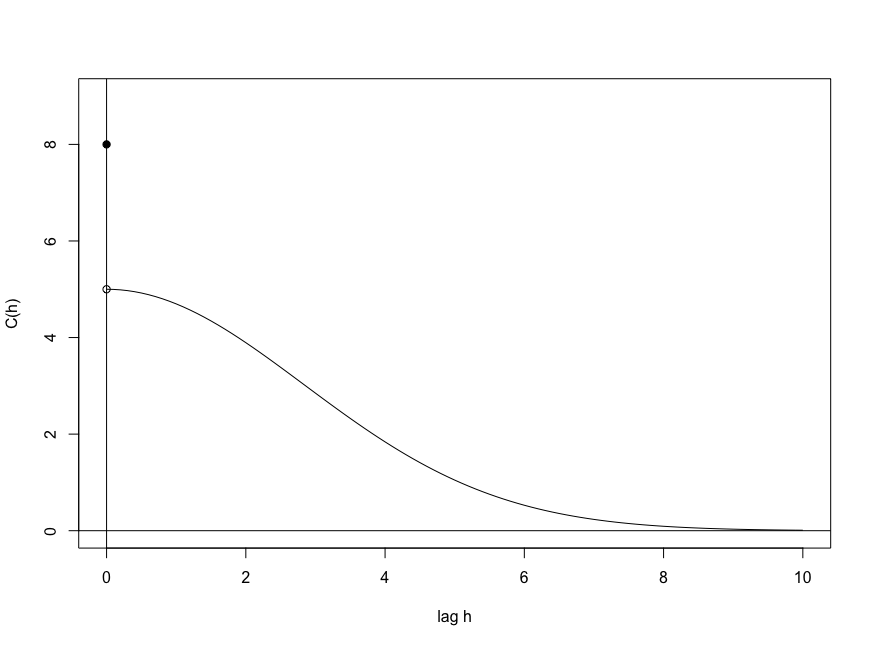
\includegraphics[width = .85\textwidth]{Rplot01.png}
        \end{center}
      \end{figure}

    \item[b.]Calculate the corresponding semivariogram. (Be sure to show your work.) You need 
    to be careful about your calculations at $h = 0$.\\
    \solution Recall the relationship between a covariogram and the corresponding semivariogram, 
    \begin{equation*}
      \gamma(h) = C(0) - C(H).
    \end{equation*}
    Applying this relationship to both parts of the piecewise function $C(h)$ we get the following, 
    \begin{align*}
      \gamma(h) &= 
      \begin{cases}
        C(0) - C(0) & h = 0\\
        C(0) - C(h) & h > 0
      \end{cases},\\
      &=
      \begin{cases}
        0 & h = 0\\
        8 - 5e^{-h^2/16} & h > 0
      \end{cases}
    \end{align*}
    Plotting the resulting semivariogram, we get the following, \\      
    \textbf{Code:}
    \begin{center}
    \lstinputlisting[basicstyle = \footnotesize]{r7.txt}
    \end{center}

    \begin{figure}[H]
      \begin{center}
      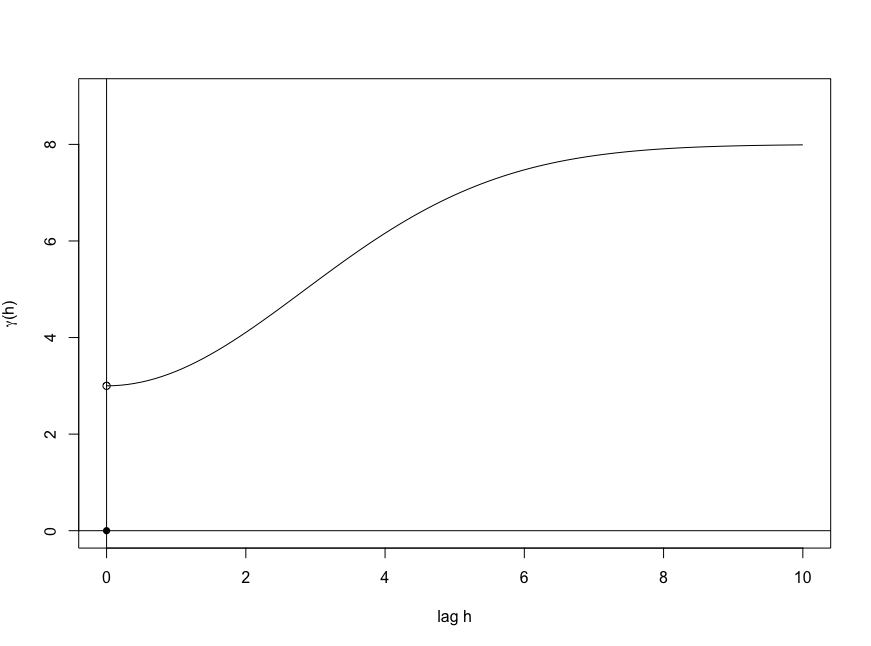
\includegraphics[width = .85\textwidth]{Rplot02.png}
      \end{center}
    \end{figure}



    \item[c.] What kind of (semi)variogram is this, and what are its parameters?\\
    \solution This is an example of an exponential semivariogram. It's parameters are $\tau^2 = 3, \sigma^2 = 5$ and $\phi = 16$. 
    \begin{align*}
      \gamma(h) &= 
      \begin{cases}
        0 & h = 0\\
        8 - 5e^{-h^2/16} & h > 0
      \end{cases},\\
      &=
      \begin{cases}
        0 & h = 0\\
        3 + 5(1 - e^{-h^2/16}) & h > 0
      \end{cases},\\
      &=
      \begin{cases}
        0 & h = 0\\
        \tau^2 + \sigma^2(1 - e^{-h^2/\phi}) & h > 0
      \end{cases}
    \end{align*}
    

    \item[d.] What is the nugget? the partial sill? the sill? the range (or effective range)? $Var(Y(s))$?\\
    \solution  From the figure we can see that the nugget for the semivariogram is 3. The partial sill is 5. The sill is 8. the 
    range looks to go from $[0,10]$ maybe even $[0,8]$. 
  \end{enumerate}
  
\end{exercise}
\vspace{.5in}



\begin{exercise}{4} Consider the semivariogram,
  \begin{equation*}
    \gamma(h) = 
    \begin{cases}
      0 & h = 0\\
      3 + 7(1.5(h/6) - .5(h/6)^3) & 0 < h < 6\\
      10 & h \geq 6
    \end{cases}
  \end{equation*}
  \begin{enumerate}
    \item[a.] Use R to sketch $\gamma(h)$ for a suitable range of $h$.\\
    \solution  \\
    \textbf{Code:}
    \begin{center}
    \lstinputlisting[basicstyle = \footnotesize]{r6.txt}
    \end{center}

    \begin{figure}[H]
      \begin{center}
      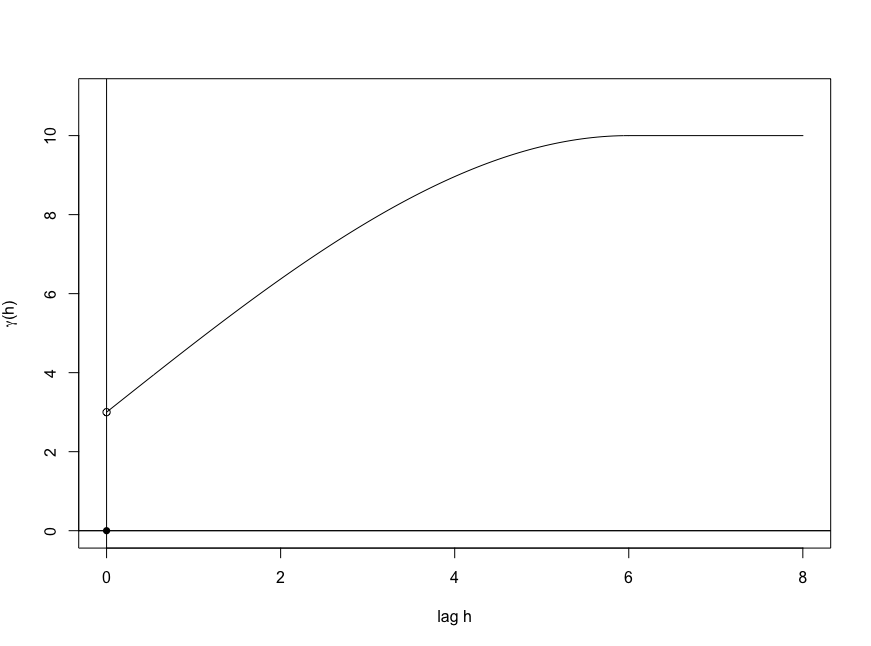
\includegraphics[width = .85\textwidth]{Rplot03.png}
      \end{center}
    \end{figure}


    \item[b.] Find the corresponding covariogram, $C(h)$. \\
    \solution Recall the relationship between a covariogram and a semivariogram, 
    \begin{equation*}
      C(h) = \lim_{R \to \infty}\gamma(R) - \gamma(h).
    \end{equation*} 
    Applying this relationship to each part of the piecewise definition of $\gamma(h)$ we get, 
    \begin{align*}
      C(h) &= \begin{cases}
        10 - 0 & h = 0,\\
        10 -  (3 + 7(1.5(h/6) - .5(h/6)^3)) & 0 < h < 6,\\
        10 - 10 & h \geq 6.
      \end{cases},\\
      &= \begin{cases}
        10 & h = 0,\\
        10-3-7(1.5(h/6) - .5(h/6)^3)) & 0 < h < 6,\\
        0 & h \geq 6.
      \end{cases}\\
      &= \begin{cases}
        10 & h = 0,\\
        7-7(\dfrac{3}{2}(h/6) - \dfrac{1}{2}(h/6)^3)) & 0 < h < 6,\\
        0 & h \geq 6.
      \end{cases}
    \end{align*}
    Plotting in R we get the following, \\
    \textbf{Code:}
    \begin{center}
    \lstinputlisting[basicstyle = \footnotesize]{r8.txt}
    \end{center}

    \begin{figure}[H]
      \begin{center}
      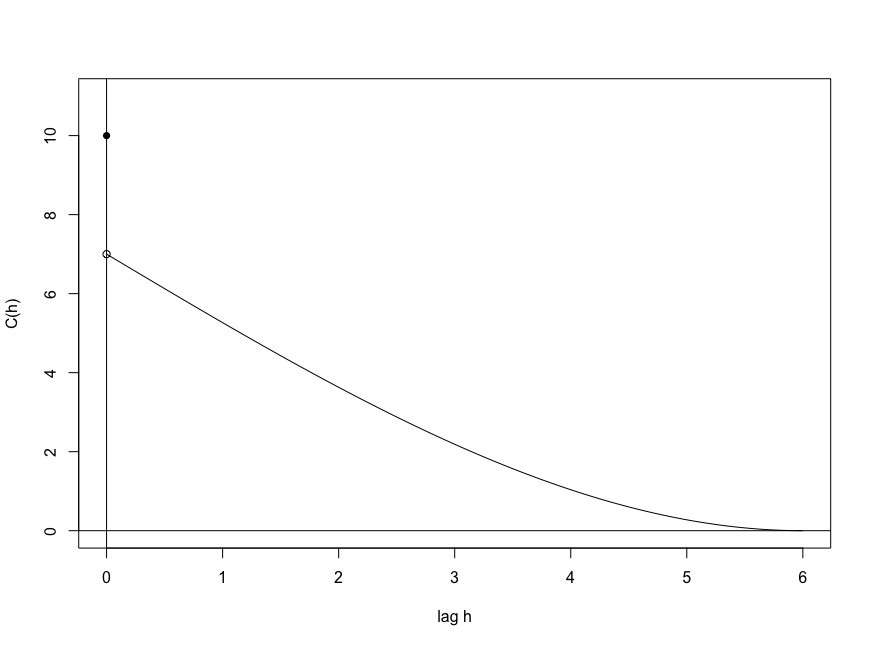
\includegraphics[width = .85\textwidth]{Rplot04.png}
      \end{center}
    \end{figure}


    




    \item[c.] What kind of (semi)variogram is this, and what are its parameters?\\
    \solution This is an example of a spherical semivariogram with parameters $\tau^2 = 3$, 
    $\sigma^2 = 6$, and $\phi = 6$. 
    \vspace{.15in}


    \item[d.] What is the nugget? the partial sill? the sill? the range? $Var(Y(s))$?\\
    \solution From the figure we can see that the nugget for the semivariogram is 3. The partial sill is 
    7. The sill is 10. The range is from $[0,6]$.
    \vspace{.15in}
  \end{enumerate}
\end{exercise}


\begin{exercise}{5} Let $X$ be a discrete random variable such that, 
  \begin{center}
    \begin{tabular}{c|| c c c c }
      $x$ & -2 & -1 & 1 & 2\\
      \hline
      $P(X = x)$ & .4 & .1 & .1 & .4\\
     \end{tabular}
    \end{center}
    Define $Y = X^2$. 
    \begin{enumerate}
      \item[a.] Show that $cov(X, Y) = 0$ (To do this, you wil need to calculate $E(X)$, $E(Y)$, and $E(XY)$, and use the formula for covariance frm page 
      25 of the lecture notes.)\\
      \solution Recall the formula for the covariance,
      \begin{equation*}
        cov(X, Y) = E(XY) - \mu_x\mu_y = E(X^3) - \mu_x\mu_y.
      \end{equation*}
      Computing each term we get, 
      \begin{equation*}
        E(X^3) = (.4)(-2)^3 + (.1)(-1)^3 + (.1)1^3 + (.4)2^3 = 0. 
      \end{equation*}
      \begin{equation*}
        \mu_x = \dfrac{(-2) + (-1) + (1) + (2)}{4} = 0.
      \end{equation*}
      \begin{equation*}
        \mu_y = \dfrac{(-2)^2 + (-1)^2 + (1)^2 + (2)^2}{4} = 2.4.
      \end{equation*}
      \begin{equation*}
        cov(X, Y) = E(X^3) - \mu_x\mu_y = 0 - 0(2.4) = 0.
      \end{equation*}
      \vspace{.15in}


      \item[b.] Show that $X$ and $Y$ are dependent. (E.g., calculate $P(X = 1, Y = 4)$ and $P(X = 1)P(Y = 4)$; if $X$ and $Y$
      are independent, these two values- among others- must be equal.)\\
      \solution Following the example described in the hint consider the following, 
      \begin{equation*}
        P(X = 1, Y = 4) = 0.
      \end{equation*}
      Since $Y = X^2$ we know that when $X = 1$ it follows that $Y = 1$ and similarly if $y = 4$ it follows that $X = 2,-2$. In anycase 
      the joint probability $P(X = 1, Y = 4)$ must be zero. Furthermore computing the product we get,
      \begin{equation*}
        P(X = 1)P(Y = 4) = (.1)(.8) = .08 \neq 0.
      \end{equation*}
      Thus $X$ and $Y$ are dependent.
    \end{enumerate}
  
  
\end{exercise}













\end{document}


















